\subsection{The Cleaning Service}
\label{sec:cleaningService}

Deliverable 3.2~\cite{d3.2} presents a description of the RESTful API of the cleaning service. 
The cleaning service contains the two methods \texttt{getCleaningSuggestions} and \texttt{clean}, of which we give an update.
The functionality of the methods  declared in the Deliverable 3.1~\cite{d3.1} remains unchanged.

The HTTP method for \texttt{getCleaningSuggestions} has been changed from POST to GET, such as the former method means retrieve information from a server, while the POST method determines changes to be done in resources, e.g. creation of new resources or updating of existing resources. Semantic of the \texttt{getCleaningSuggestions} does not foresee any manipulation on resources, in our case it is an update of \texttt{RDF} data.
The parameters of the GET request method were slightly changed. The response of the \texttt{getCleaningSuggestions} GET request were extended in order to address flows in case of passing illegal or incorrect parameters. The detail description of the GET request and response provided bellow.

The cleaning part of the exposed web service was implemented what led to updates of the POST request and response parameters regarding to the Deliverable 3.1~\cite{d3.1}.


The typical usage of the cleaning service follows the workflow outlined for the cleaning application in figure \ref{fig:workflow}.
The updated user interface is shown in figure \ref{fig:ui}

\begin{figure}[ht!]
\centering
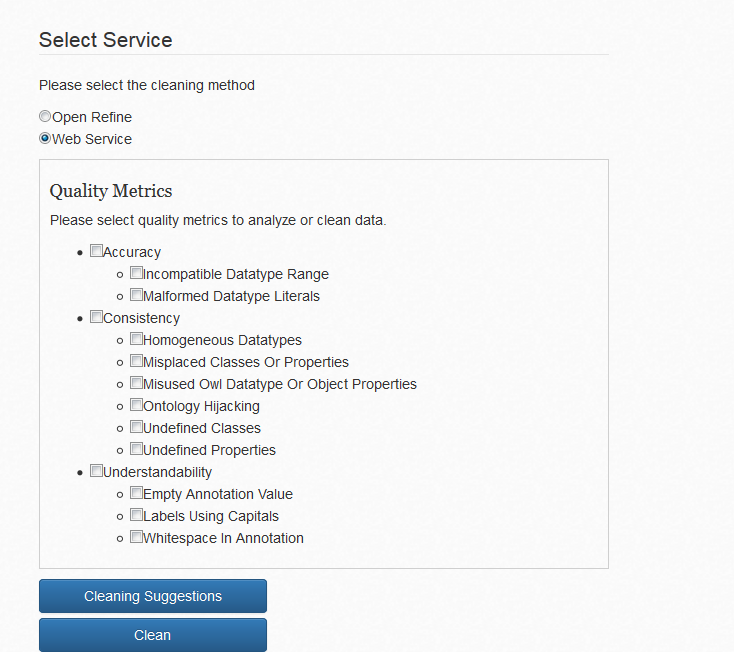
\includegraphics[width=\textwidth]{figures/WebService.png}
\caption{Cleaning process workflow}
\label{fig:ui}
\end{figure}





\subsubsection{Exposed Web Service Interfaces}
\label{sec:service-API}


\begin{table}[h]
\captionsetup{justification=raggedright,singlelinecheck=false}
\caption{Cleaning Methods}
\label{tbl:valid_meth}
\begin{tabular}{|p{5cm}|p{10cm}|}
\hline
\multicolumn{2}{|l|}{\textbf{Methods}} \\ \hline

\textbf{Modifier and Type} & 
\textbf{Method and Description} \\ \hline

\texttt{HttpServletRequest} & 
\texttt{getCleaningSuggestionsREST(HttpServletRequest
request, HttpServletResponse response)}: \textbf{GET} method which returns a set of cleaning suggestions. \\ \hline

\texttt{HttpServletRequest} & 
\texttt{cleanREST(HttpServletRequest
request, HttpServletResponse response)}: \textbf{POST} method which removes triples affected by selected quality problems. \\ \hline

\hline
\end{tabular}
\end{table}
Note: HttpServletRequest and HttpServletResponse are interfaces of the javax.servlet.http package.

\subparagraph{Method Details}

\begin{description}

\item{\textbf{getCleaningSuggestionsJSON}:} \textbf{REST} method which returns a set of cleaning suggestions.

\textbf{URL (partial):} \url{/quality_extension/get_cleaning_suggestions} 

\textbf{Parameters}: 
\begin{itemize}
\item \texttt{HTTP Request message}: A JSON-encoded string which has the following structure: \\
\hspace*{0.2 cm}\{\\
\hspace*{0.5 cm}"download": "Dataset", \\
\hspace*{0.5 cm}"metrics": ["metric1", "metric2"]  \\
\hspace*{0.2 cm}\} \\
\end{itemize}
Where
\begin{description}
\item[download:] The URI of a file to be validated. 
\item[metrics:] A list of quality metrics metrics is list of metrics with respect to which cleaning suggestions should be generated. 
\end{description}


\textbf{Returns}: A Response instance which has a \texttt{JSON} encoded entity content depending on the input parameter of the method. We discriminate the following cases: 
\begin{itemize}
\item  HTTP status code 400 and the entity content, if the input parameters or one of them are empty:\\ \hspace*{0.2 cm}\{\\
\hspace*{0.5 cm} "status" : "error",\\
\hspace*{0.5 cm} "message" : "Request parameters are not complete."\\ \hspace*{0.2 cm} \}

\item  HTTP status code 200 and the entity content, if the input parameters are correct and the get cleaning suggestion method has not fail:\\ \hspace*{0.2 cm} \{\\
 \hspace*{0.5 cm}"status" : "ok",\\ 
 \hspace*{0.5 cm}  "message" : "Quality report in one of \texttt{RDF} serialisations." \\ \hspace*{0.2 cm} \}

\item HTTP status code 400 and the entity content, if the input parameters are not correct:\\ \hspace*{0.2 cm} \{ \\
\hspace*{0.5 cm} "status" : "error",\\
\hspace*{0.5 cm}  "message" : "Request parameters cannot be parsed."\\ \hspace*{0.2 cm} \}

\end{itemize}
The cleaning report is created according to the QR (Quality Report) and QPROB (Quality Problems) ontologies presented in Deliverable 3.2~\cite{d3.2}.
An example of the cleaning report is shown in Figure \ref{lst:cleaning_report}.


We also extended cleaning report by statistics that summarize information about identified quality problems and affected triples. 
The QR ontologie were extended by the corresponding classes and properties represented in Figure \ref{fig:stat}


\begin{figure}[ht!]
\centering
\includegraphics[page=8,trim=1.0cm 1.0cm 1.0cm 1.0cm,clip,width=\textwidth]{figures/CleaningFigures.pdf}
\caption{Quality Statistics in Quality Report Ontology}
\label{fig:stat}
\end{figure}
\lstinputlisting[caption={An example of a cleaning report},label=lst:cleaning_report]{figures/cleaning_report.trig}


\item{\textbf{clean}:} \textbf{POST} method which which cleans a dataset by applying the rule ``delete every triple that is affected by a quality problem w.r.t.\ to at least one of the metrics specified''.

\textbf{URL (partial):} \url{/quality_extension/clean} 

\textbf{Parameters}: 
\begin{itemize}
\item \texttt{HTTP Request message}: A JSON encoded string which has the following structure: \\
\{ \\
\hspace*{0.5 cm}"download": "Dataset", \\
\hspace*{0.5 cm}"metrics": ["metric1", "metric2"], \\
\hspace*{0.5 cm}"delta": "true | false" \\  
\} \\

Where 
\begin{description}
\item[Dataset:] The URI of an \texttt{RDF} file to be validated. 
\item[metrics:] A list of metrics with respect to which cleaning suggestions should be generated.
\end{description}

\end{itemize}
\textbf{Returns}: A Response instance which has a JSON encoded entity content depending on the input parameter of the method. We discriminate the following cases: 
\begin{itemize}
\item  HTTP status code 400 and the entity content, if the input parameters or one of them are empty:\\ \hspace*{0.2 cm}\{\\
\hspace*{0.5 cm} "status" : "error",\\
\hspace*{0.5 cm} "message" : "Request parameters are not complete."\\ \hspace*{0.2 cm} \} 

\item HTTP status code 400 and the entity content, if the input parameters are not correct:\\ \hspace*{0.2 cm} \{ \\
\hspace*{0.5 cm} "status" : "error",\\
\hspace*{0.5 cm}  "message" : "Request parameters cannot be parsed or an error occurred while applying metrics."\\ \hspace*{0.2 cm} \}

\item  HTTP status code 200 and the entity content, if the input parameters are correct and the get cleaning suggestion method has not fail: \\ \hspace*{0.2 cm} \{\\ \hspace*{0.5 cm} "status" : "ok",\\ \hspace*{0.5 cm} "uri":  "Cleaned \texttt{RDF} data serialized in TURTLE.", \\ \hspace*{0.5 cm}"delta" : "Removed \texttt{RDF} statements serialized in TURTLE." \\ \hspace*{0.2 cm}\} 

\todo{@Christoph originally it was said to return cleaned rdf data in some serialization for the "uri" key, i have implement it like that, but i think you should implement some assets storage within the extension and extend the rest api for retrieving the data, then we can return only uri}
\end{itemize}

\end{description}






\

%%% Local Variables: 
%%% mode: latex
%%% TeX-master: "D3.2"
%%% End: 
